\documentclass[aspectration=1610,t]{beamer}
\usepackage{csc}
\title{Лекция 3. OpenGL --- векторные преобразования}


\date{
   \textbf{ИТМО}\\
   28 сентября 2022\\
   Санкт-Петербург
}

\begin{document}

\begin{frame}
  \titlepage
\end{frame}

\begin{frame}[fragile]{Вектора}
    Самые "распространненые/используемые" алгебраические структуры:
    \begin{itemize}
        \item {\bf вектора} - направленные отрезки (размерности 2, 3 или 4);
        \item {\bf матрицы} - таблицы (как правило квадратные), размерности $2x2$, $3x3$, $4x4$.
    \end{itemize}
    Операции:
    \begin{itemize}
        \item {\bf скаляр-вектор}
        \item {\bf вектор-вектор}
        \item {\bf матрица-вектор}
    \end{itemize}
\end{frame}

\begin{frame}[fragile]{Операции со скалярами}
    Примеры:
    \begin{itemize}
        \item Умножение на скаляр: $(x, y, z) \cdot \alpha = (\alpha \cdot x, \alpha \cdot y, \alpha \cdot z)$
        \item Сложение скаляра: $(x, y, z) + \alpha = (\alpha + x, \alpha + y, \alpha + z)$
        \item Обратный вектор: $-(x, y, z) = (-x, -y, -z)$
        \item ...
    \end{itemize}
\end{frame}

\begin{frame}[fragile]{Операции c векторами и матрицами}
    Примеры:
    \begin{itemize}
        \item Сложение: $(x, y, z) + (a, b, c) = (x + a, y + b, z + c)$
        \item Длина: $len (x, y, z) = \sqrt{x^2 + y^2 + z^2}$
        \item Нормализация: $normalize (x, y, z) = \frac{(x, y, z)}{ len (x, y, z)}$
        \item Скалярное произведение: $(x, y, z) \cdot (a, b, c) = x \cdot a + y \cdot b + z \cdot c$
        \item Векторное произведение: $(x, y, z) \times (a, b, c) = (y \cdot c - z \cdot b, z \cdot a - x \cdot c, x \cdot b - y \cdot a)$
        \item Умножение: $\begin{bmatrix} a & b \\ c & d \\ \end{bmatrix} \times (x, y) = (a \cdot x + c \cdot y, b \cdot x + d \cdot y)$
        \item ...
    \end{itemize}
\end{frame}

\begin{frame}[fragile]{Полезные преобразования}
    \begin{itemize}
        \item
        $
        \begin{bmatrix}
            sx & 0 & 0 & 0 \\
            0 & sy & 0 & 0 \\
            0 & 0 & sz & 0 \\
            0 & 0 & 0 & 1 \\
        \end{bmatrix}
        \times
        \begin{bmatrix}
            x \\
            y \\
            z \\
            1 \\
        \end{bmatrix}
        =
        \begin{bmatrix}
            x \cdot sx \\
            y \cdot sy \\
            z \cdot sz \\
            1 \\
        \end{bmatrix}
        $
        \item
        $
        \begin{bmatrix}
            1 & 0 & 0 & dx \\
            0 & 1 & 0 & dy \\
            0 & 0 & 1 & dz \\
            0 & 0 & 0 & 1 \\
        \end{bmatrix}
        \times
        \begin{bmatrix}
            x \\
            y \\
            z \\
            1 \\
        \end{bmatrix}
        =
        \begin{bmatrix}
            x + dx \\
            y + dy \\
            z + dz \\
            1 \\
        \end{bmatrix}
        $
        \item
        $
        \begin{bmatrix}
            1 & 0 & 0 & dx \\
            0 & cos(\alpha) & -sin(\alpha) & dy \\
            0 & -sin(\alpha) & cos(\alpha) & dz \\
            0 & 0 & 0 & 1 \\
        \end{bmatrix}
        \times
        \begin{bmatrix}
            x \\
            y \\
            z \\
            1 \\
        \end{bmatrix}
        =
        \begin{bmatrix}
            x \\
            y \cdot cos(\alpha) - z \cdot sin(\alpha) \\
            y \cdot cos(\alpha) + z \cdot cos(\alpha) \\
            1 \\
        \end{bmatrix}
        $
        \item + комбинации преобразований ({\bf важен порядок!})
    \end{itemize}
\end{frame}

\begin{frame}[fragile]{На практике}
    Упрощение работы с математикой:
    \begin{itemize}
        \item Средства {\bf QT}:
        {\small \begin{lstlisting}
QMatrix4x4 matrix;
matrix.perspective(60.0, 4.0 / 3.0, 0.1, 100.0);
matrix.translate(0, 0, -2);
matrix.rotate(90., rotation_axis);
        \end{lstlisting}}
        \item Библиотека {\bf GLM}
        {\small \begin{lstlisting}
glm::mat4 trans;
auto pos = glm::vec3(0.0, 0.0, 1.0);
trans = glm::rotate(trans, 90.0, pos);
trans = glm::scale(trans, glm::vec3(0.5, 0.5, 0.5));  
                        \end{lstlisting}}
        \item Другие библиотеки...
    \end{itemize}
\end{frame}

\begin{frame}[fragile]{Еще раз о преобразовании координат}
    \begin{figure}[htp]
        \centering
        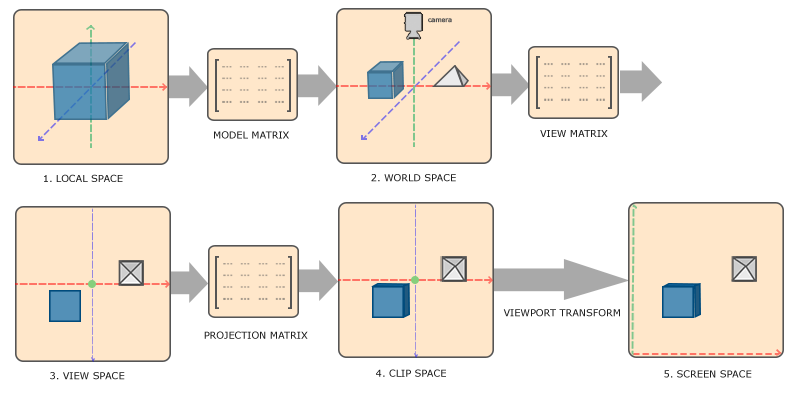
\includegraphics[scale=0.40]{res/coord}
    \end{figure}
\end{frame}

\begin{frame}[fragile]{Камера}
    \begin{figure}[htp]
        \centering
        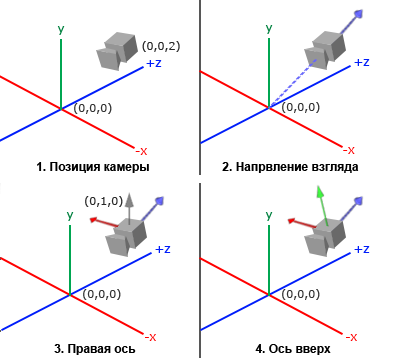
\includegraphics[scale=0.40]{res/cam}
    \end{figure}
    Задается 3 векторами, которые образуют новую СК, начало СК совпадает с положением камеры.
\end{frame}

\begin{frame}[fragile]{Как задать камеру}
    Положение
            {\small \begin{lstlisting}
glm::vec3 cameraPos = glm::vec3(0.0f, 0.0f, 3.0f);
            \end{lstlisting}}

    Направление взгляда
        {\small \begin{lstlisting}
glm::vec3 cameraTarget = glm::vec3(0.0f, 0.0f, 0.0f);
glm::vec3 cameraDirection = glm::normalize(cameraPos 
    - cameraTarget);
        \end{lstlisting}}

    Вектор вправо
        {\small \begin{lstlisting}
glm::vec3 up = glm::vec3(0.0f, 1.0f, 0.0f); 
glm::vec3 cameraRight = glm::normalize(
    glm::cross(up, cameraDirection));
        \end{lstlisting}}
    
    Вектор вверх
        {\small \begin{lstlisting}
glm::vec3 cameraUp = glm::cross(cameraDirection,
    cameraRight);
        \end{lstlisting}}
\end{frame}

\begin{frame}[fragile]{lookAt}
    Математика преобразований:

    $
        \begin{bmatrix}
            R_x & R_y & R_z & 0 \\
            U_x & U_y & U_z & 0 \\
            D_x & D_y & D_z & 0 \\
            0 & 0 & 0 & 1 \\
        \end{bmatrix}
        \times
        \begin{bmatrix}
            1 & 0 & 0 & X \\
            0 & 1 & 0 & Y \\
            0 & 0 & 1 & Z \\
            0 & 0 & 0 & 1 \\
        \end{bmatrix}
        = [...]
    $ - look at matrix

    В коде же:
            {\small \begin{lstlisting}
glm::mat4 view;
view = glm::lookAt(glm::vec3(0.0f, 0.0f, 3.0f), 
    glm::vec3(0.0f, 0.0f, 0.0f), 
    glm::vec3(0.0f, 1.0f, 0.0f));
            \end{lstlisting}}
\end{frame}

\end{document}

